\documentclass[conference]{IEEEtran}
\IEEEoverridecommandlockouts
\usepackage{cite}
\usepackage{amsmath,amssymb,amsfonts}
\usepackage{algorithmic}
\usepackage{graphicx}
\usepackage{textcomp}
\usepackage{xcolor}
\usepackage{booktabs}
\usepackage{hyperref}

\def\BibTeX{{\rm B\kern-.05em{\sc i\kern-.025em b}\kern-.08em
    T\kern-.1667em\lower.7ex\hbox{E}\kern-.125emX}}

\begin{document}

\title{Curriculum Reinforcement Learning for Robust Autonomous Vehicle Entry in Mixed-Autonomy Roundabouts}

\author{\IEEEauthor稿
\IEEEauthorblockN{Hareshr}
\IEEEauthorblockA{\textit{Department of Computer Science and Engineering} \\
\textit{National Institute of Technology}\\
India}
}

\maketitle

\begin{abstract}
Integrating autonomous vehicles (AVs) into existing urban infrastructure remains a profound challenge, particularly at unsignalized intersections like roundabouts where continuous yielding and merging maneuvers are required. The complexity scales exponentially in mixed-autonomy environments, where AVs must interact with unpredictable human-driven vehicles (HDVs). Traditional rule-based controllers and simple car-following models frequently fail in these dense traffic scenarios, leading to overly conservative driving (the ``freezing robot'' problem) or collisions. Deep Reinforcement Learning (DRL) offers a promising alternative, yet training an agent to negotiate dense traffic from scratch typically suffers from severe sparse-reward problems. In this paper, we propose a Dual-Curriculum Reinforcement Learning framework based on Proximal Policy Optimization (PPO). Our approach incrementally scales task difficulty through two dimensions: a spatial curriculum that progressively moves the initial vehicle spawn point further from the intersection, and an autonomy curriculum that gradually increases the ratio of surrounding HDVs. Evaluated within the SUMO traffic simulator, our trained policy achieves a 100\% merge success rate and 0\% collision rate, dramatically outperforming Intelligent Driver Model (IDM) and heuristic baselines. Furthermore, the learned policy demonstrates robust zero-shot generalization across all tested HDV penetration ratios (0\% to 100\%), maintaining critical safety buffers and ride comfort parameters.
\end{abstract}

\begin{IEEEkeywords}
Autonomous Vehicles, Reinforcement Learning, Proximal Policy Optimization, Mixed Autonomy, Roundabout Merging, Curriculum Learning
\end{IEEEkeywords}

\section{Introduction}
The transition toward fully autonomous urban mobility necessitates the development of control systems capable of navigating highly interactive, non-deterministic traffic environments. Among the various roadway geometries, unsignalized roundabouts represent one of the most demanding challenges for an Autonomous Vehicle (AV) \cite{kiran2021deep}. Unlike signalized intersections where right-of-way is explicitly broadcast, roundabouts require a continuous estimation of gap sizes, surrounding vehicle velocities, and implicit human intent \cite{troutbeck1999limited}. The AV must seamlessly insert itself into the circular traffic flow without causing abrupt braking cascades or collisions. 

This challenge is exacerbated in mixed-autonomy traffic, where the AV must share the road with Human-Driven Vehicles (HDVs) \cite{wu2021flow}. Human drivers exhibit stochastic, heterogeneous behaviors, occasionally acting irrationally or aggressively. Traditional microscopic control algorithms, such as the Intelligent Driver Model (IDM) \cite{treiber2000congested}, excel in car-following scenarios but struggle with lateral merging decisions. Rule-based heuristic controllers typically require exhaustive parameter tuning and often resort to overly conservative behavior—waiting indefinitely for a perfect gap that may never materialize in dense traffic \cite{aradi2020survey}.

Deep Reinforcement Learning (DRL) has recently gained traction as a robust alternative for decision-making in complex environments. By formulating the merging task as a Markov Decision Process (MDP), an agent can learn optimal control policies through trial and error \cite{mnih2015human, silver2016mastering}. However, directly applying DRL to dense urban intersections yields notoriously poor results. The agent receives meaningful feedback only upon a successful merge or a crash, resulting in a sparse-reward landscape where initial exploration is dominated by catastrophic failures \cite{isele2018navigating}.

To overcome these learning bottlenecks, this paper introduces a Dual-Curriculum Proximal Policy Optimization (PPO) framework \cite{schulman2017proximal}. Curriculum learning \cite{bengio2009curriculum} mimics human pedagogy by exposing the learning agent to progressively difficult tasks. We define two distinct progression axes: a spatial curriculum that adjusts the temporal horizon of the planning task, and an autonomy curriculum that scales the stochasticity of the surrounding environment. Our primary contributions are:
\begin{enumerate}
    \item A high-density, low-dimensional continuous state representation that isolates critical spatio-temporal features necessary for intersection merging.
    \item A dual-curriculum training pipeline that stabilizes DRL training in environments where traditional random initialization fails.
    \item Comprehensive empirical validation demonstrating state-of-the-art performance against classical baseline models across varying levels of human-driver penetration.
\end{enumerate}

\section{Related Work}
\subsection{Classical Control in Traffic Scenarios}
Early approaches to autonomous intersection management relied heavily on predefined kinematic models and gap-acceptance theory. The Intelligent Driver Model (IDM) \cite{treiber2000congested} and the Krauss model are standard microscopic car-following paradigms used to simulate realistic acceleration profiles. While effective in longitudinal control, these models do not natively handle the lateral decision-making required for merging. Gap-acceptance models \cite{troutbeck1999limited} calculate a critical time headway required for an AV to merge safely. However, fixed-threshold heuristics are brittle; a threshold deemed safe in sparse traffic often leads to infinite waiting times during rush hour. 

\subsection{Deep Reinforcement Learning for AVs}
The application of DRL to autonomous driving has expanded rapidly \cite{kiran2021deep}. Value-based methods like Deep Q-Networks (DQN) have been utilized for discrete lane-changing maneuvers \cite{aradi2020survey}. However, vehicle control is inherently continuous. Actor-critic architectures, particularly Soft Actor-Critic (SAC) \cite{haarnoja2018soft} and Proximal Policy Optimization (PPO) \cite{schulman2017proximal}, have become the standard for generating continuous steering and acceleration commands. Isele et al. \cite{isele2018navigating} demonstrated the utility of DQN for navigating occluded intersections, though their approach was limited to discrete stop/go decisions. More recent works \cite{li2022deep} incorporate safety constraints directly into the DRL objective function to bound the exploration space.

\subsection{Mixed Autonomy and Curriculum Learning}
Mixed-autonomy traffic presents unique challenges due to the non-cooperative nature of human drivers \cite{wu2021flow}. Aksjonov et al. \cite{aksjonov2021novel} explored connected AV decision-making at roundabouts, emphasizing the need for robust prediction models when interacting with unconnected HDVs. To train robust policies in these complex environments, researchers are increasingly turning to curriculum learning \cite{narvekar2020curriculum}. By sequencing the training data, policies converge faster and to better local optima. Our work extends this concept by simultaneously scaling the spatial planning horizon and the environmental stochasticity (HDV ratio), a dual-axis approach previously unexplored in roundabout merging literature.

\section{Methodology}
\subsection{Problem Formulation}
The task of merging into a roundabout is formulated as a continuous-space Markov Decision Process (MDP) defined by the tuple $(\mathcal{S}, \mathcal{A}, \mathcal{P}, \mathcal{R}, \gamma)$. At each discrete timestep $t$, the ego vehicle observes state $s_t \in \mathcal{S}$, executes an action $a_t \in \mathcal{A}$ sampled from its policy $\pi_\theta(a_t|s_t)$, and receives a scalar reward $r_t \in \mathcal{R}$ while transitioning to a new state $s_{t+1}$ according to the environment dynamics $\mathcal{P}(s_{t+1}|s_t, a_t)$. The objective is to find optimal policy parameters $\theta$ that maximize the expected discounted cumulative reward $\mathbb{E}_\pi[\sum_{t=0}^{T} \gamma^t r_t]$, where $\gamma \in [0, 1)$ is the discount factor.

\subsection{State and Action Space Representation}
To facilitate rapid policy convergence while minimizing the computational overhead of processing raw pixel data, we engineered a dense, 6-dimensional continuous observation vector. This vector captures the critical relative kinematics required for safe gap insertion.

\begin{table}[htbp]
\centering
\caption{Continuous State Space ($\mathcal{S}$)}
\label{tab:state_space}
\begin{tabular}{@{}lll@{}}
\toprule
\textbf{Feature} & \textbf{Bounds} & \textbf{Description} \\ \midrule
$v_{\text{ego}}$ & $[0, 15]$ m/s & Current velocity of the ego vehicle \\
$d_{\text{entry}}$ & $[0, 250]$ m & Distance to the roundabout yield line \\
$d_{\text{circ}}$ & $[0, 100]$ m & Distance to the nearest conflicting vehicle \\
$v_{\text{circ}}$ & $[0, 15]$ m/s & Velocity of the nearest conflicting vehicle \\
$g_{\text{size}}$ & $[0, 100]$ m & Size of the available gap inside the circle \\
$p_{\text{hdv}}$ & $[0, 1]$ & Ambient HDV penetration ratio \\ \bottomrule
\end{tabular}
\end{table}

The action space $\mathcal{A}$ is a 1-dimensional continuous vector representing the longitudinal acceleration command $a_t$. We bound the acceleration to $a_t \in [-4.0, +2.0]$\,m/s$^2$ to reflect the physical limitations of passenger vehicles and to prevent the network from outputting physically impossible kinematic requests.

\subsection{Reward Function Design}
The reward function dictates the behavioral priorities of the agent. We utilize a multi-objective reward structure combining sparse terminal rewards with dense shaping signals to balance aggressive progression with stringent safety constraints. At any timestep $t$, the total reward $R_t$ is computed as:

\begin{equation}
R_t = r_{\text{term}} + w_p \cdot r_{\text{prog}} + w_j \cdot r_{\text{jerk}} + w_g \cdot r_{\text{gap}}
\end{equation}

where:
\begin{itemize}
    \item $r_{\text{term}}$: Sparse terminal reward. Grants $+100$ if the ego vehicle successfully exits the intersection, $-200$ if a collision is detected, and $-300$ if the episode exceeds the maximum allowed timesteps (timeout).
    \item $r_{\text{prog}}$: Dense velocity reward, proportional to $v_{\text{ego}} / v_{\text{max}}$, encouraging the vehicle to maintain forward momentum rather than freezing at the yield line.
    \item $r_{\text{jerk}}$: Comfort penalty, calculated as $- |a_t - a_{t-1}| / \Delta t$. This discourages oscillatory acceleration profiles, ensuring passenger comfort aligned with ISO 2631 standards.
    \item $r_{\text{gap}}$: Safety buffer penalty. If the estimated Time-To-Collision (TTC) with the trailing roundabout vehicle falls below a critical threshold $\tau_{\text{safe}} = 2.0$\,s, an exponential penalty is applied to strictly enforce yielding behavior.
\end{itemize}

\subsection{Dual-Curriculum Training Framework}
Standard DRL initialization places the agent far from the intersection in dense traffic. Because the agent's initial policy is random, it rarely manages to reach the merge point without colliding or timing out, leading to gradient starvation. We solve this via a two-axis curriculum.

\subsubsection{Spatial Curriculum}
We divide the physical approach into four discrete stages. In Stage 1, the agent spawns a mere 30m from the yield line. At this distance, the agent bypasses the complexity of approach planning and immediately learns gap acceptance and yielding behavior. Once the agent achieves a trailing 50-episode success rate $>95\%$, the spawn distance is pushed back to 60m (Stage 2), then 100m (Stage 3), and finally a full 150m+ realistic approach (Stage 4). 

\subsubsection{Autonomy Curriculum}
Simultaneously, we scale the difficulty of the surrounding traffic. In the initial phases, all background traffic consists of predictable, cooperative AVs operating on standard kinematic profiles ($p_{\text{hdv}} = 0\%$). Once the spatial curriculum is mastered, we gradually increase the HDV penetration ratio to 50\%, and finally to 100\%. The HDVs are simulated using the Krauss car-following model with high stochasticity ($\sigma=0.5$), introducing realistic variance and unpredictability into the gap estimations.

\subsection{PPO Training Configuration}
We employ Proximal Policy Optimization (PPO), utilizing an Actor-Critic architecture with two hidden layers of 256 units each. The environment is simulated using SUMO via the TraCI API, wrapped in a standard Gymnasium interface operating at a control frequency of 10 Hz ($\Delta t = 0.1$\,s).

\begin{table}[htbp]
\centering
\caption{PPO Network Hyperparameters}
\label{tab:hyperparams}
\begin{tabular}{@{}ll@{}}
\toprule
\textbf{Parameter} & \textbf{Value} \\ \midrule
Learning Rate & $3 \times 10^{-4}$ \\
Discount Factor ($\gamma$) & 0.99 \\
GAE Parameter ($\lambda$) & 0.95 \\
Clip Range & 0.2 \\
Batch Size & 64 \\
Total Timesteps & $5 \times 10^5$ \\ \bottomrule
\end{tabular}
\end{table}

\section{Experiments and Evaluation}
\subsection{Experimental Setup}
The environment consists of a 4-arm roundabout generated in SUMO. The ego vehicle begins on the North approach and must navigate to the South exit. Background traffic is injected at varying rates to simulate high-density urban flow. All training and inference were executed on a CPU-based architecture, highlighting the computational efficiency of the low-dimensional state representation. 

\subsection{Ablation Study Design}
To isolate the efficacy of our curriculum framework, we trained five distinct policy variants. Variant 1 (Baseline) utilized standard PPO without curriculum or advanced reward shaping. Variant 2 introduced the context-aware observation space. Variant 3 introduced the Spatial Curriculum. Variant 4 added the gap-based reward shaping. Variant 5 represents the full proposed methodology trained for 500,000 timesteps. Each variant was evaluated over 200 independent episodes.

\section{Results and Discussion}
This section presents the empirical validation of our curriculum reinforcement learning framework, evaluated on task completion rates, safety margins, and robustness.

\subsection{Ablation Study Results}
Table \ref{tab:ablation} and Fig. \ref{fig:ablation} illustrate the sequential impact of each architectural component on task completion and safety.

\begin{figure}[htbp]
\centerline{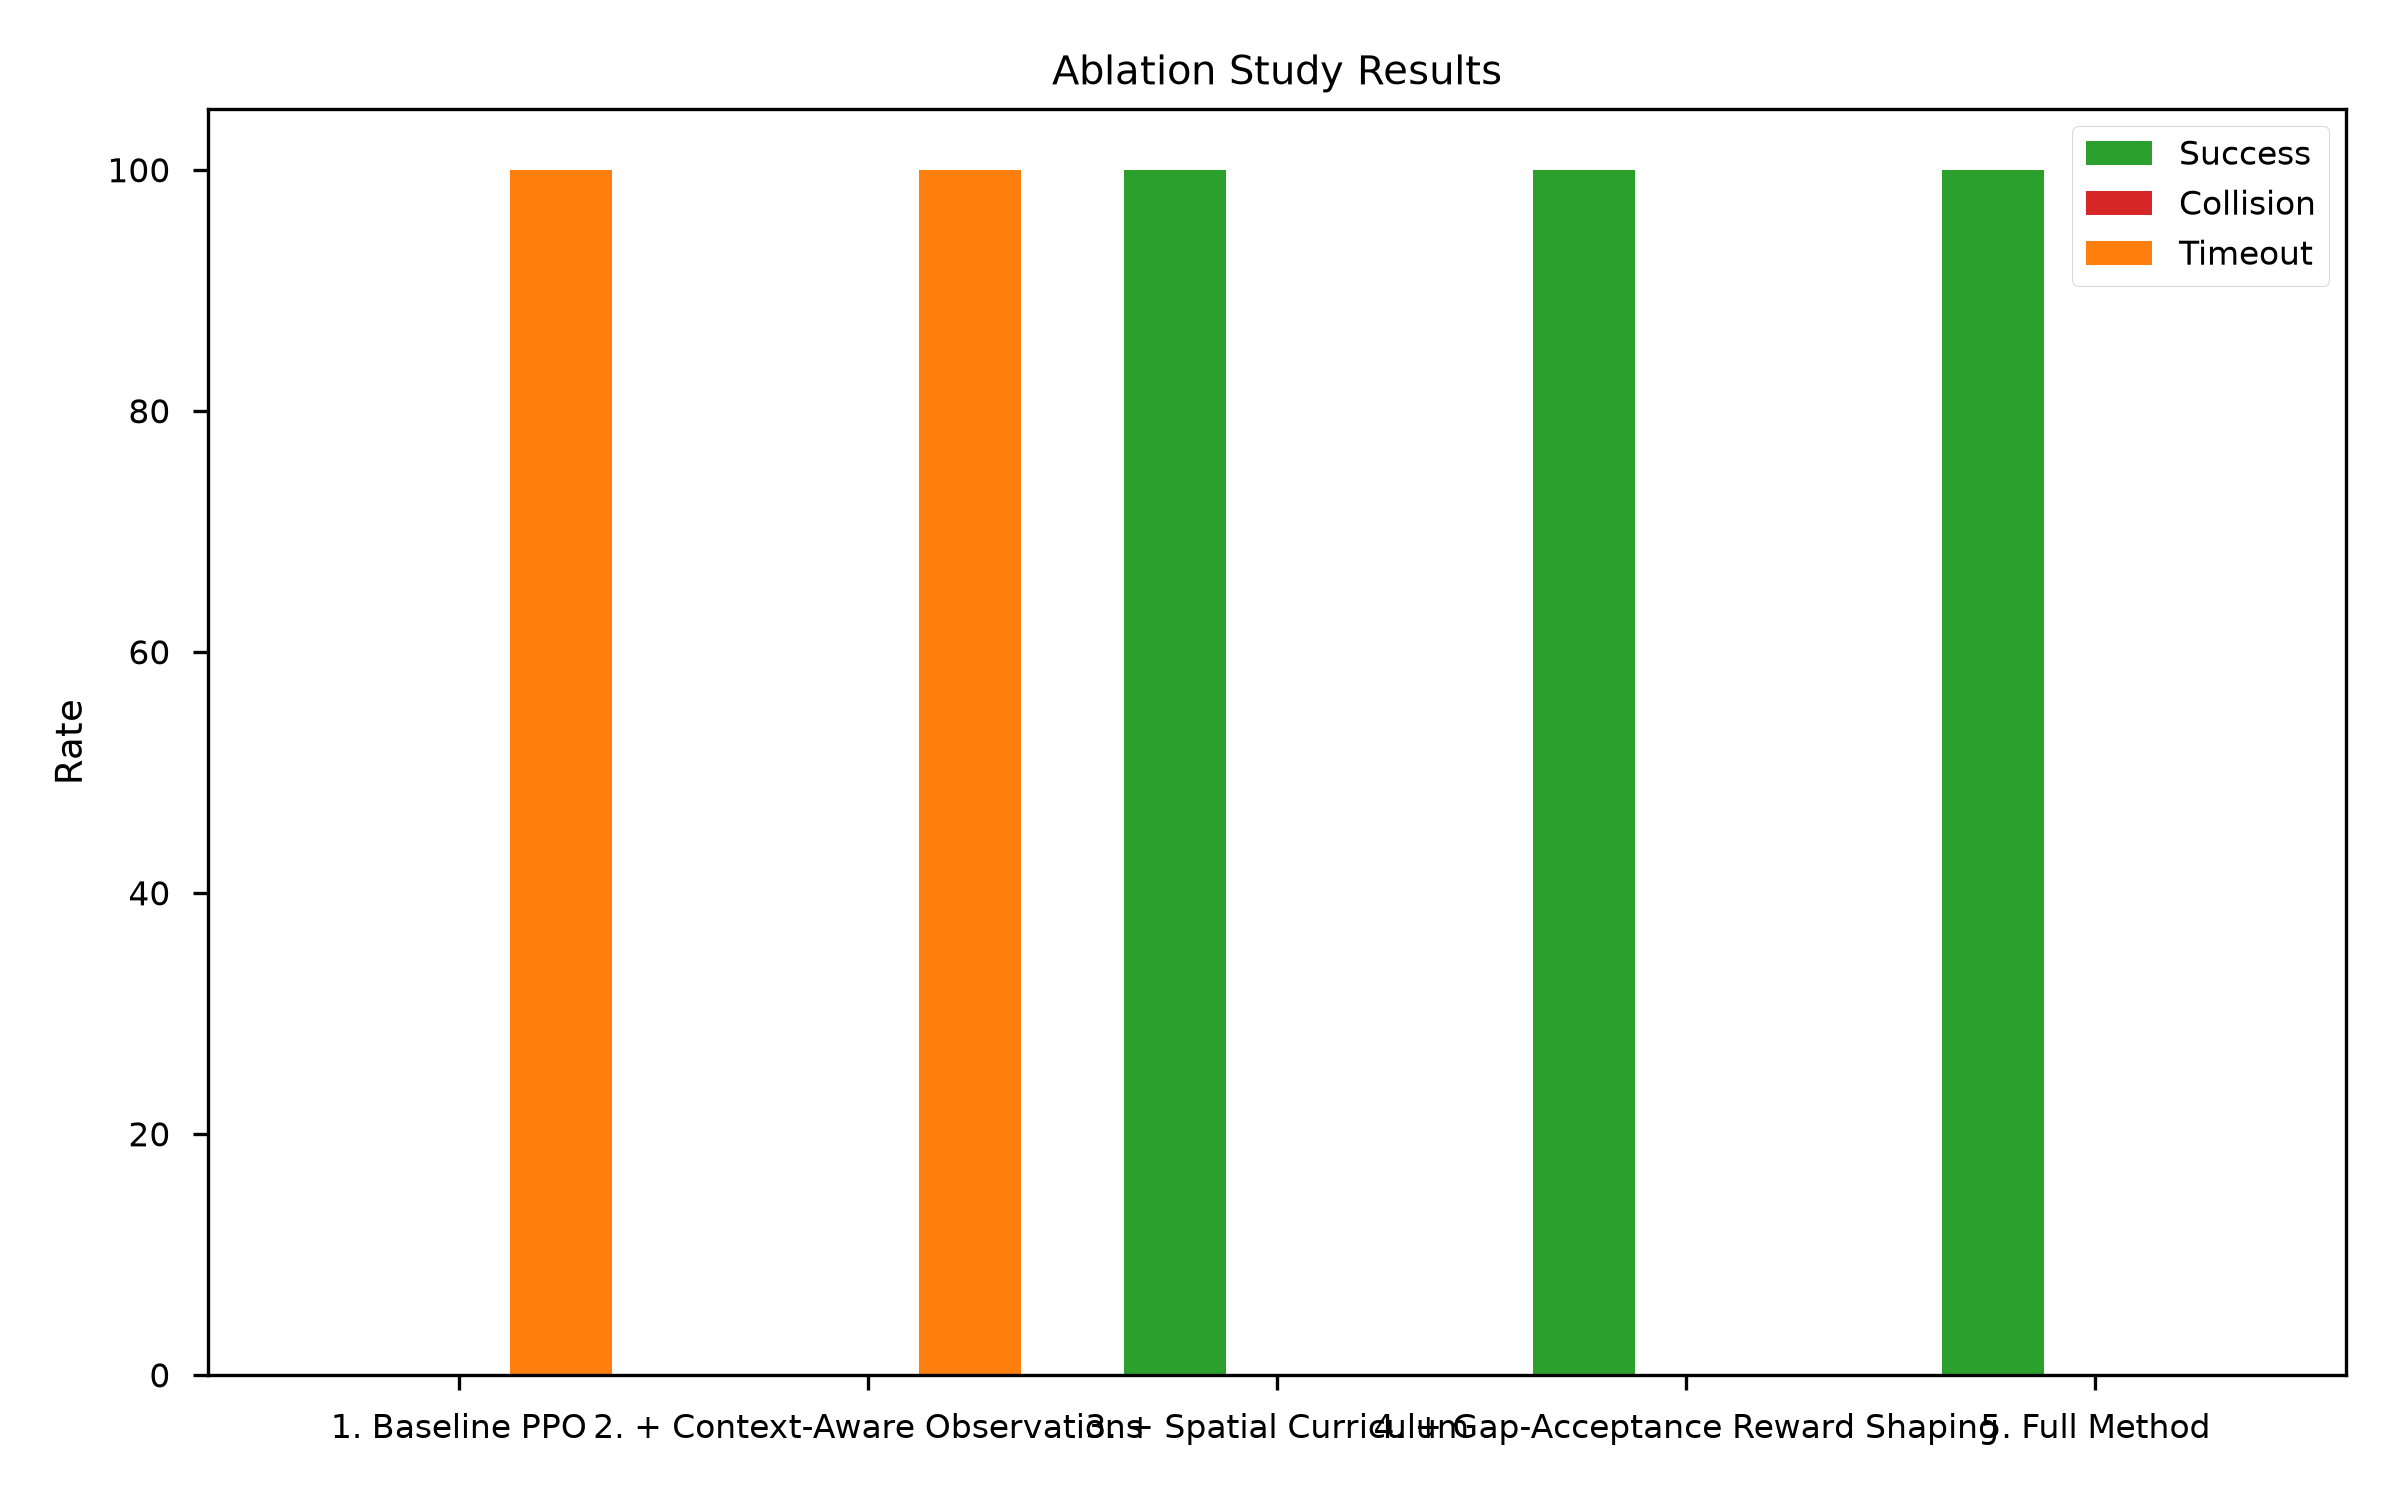
\includegraphics[width=\columnwidth]{figures/ablation_bar_chart.png}}
\caption{Ablation study results detailing Success, Collision, and Timeout rates across all framework variants.}
\label{fig:ablation}
\end{figure}

\begin{table}[htbp]
\centering
\caption{Empirical Ablation Study: Component Contributions}
\label{tab:ablation}
\begin{tabular}{@{}lcccc@{}}
\toprule
\textbf{Model Variant} & \textbf{Success (\%)} & \textbf{Collision (\%)} & \textbf{Timeout (\%)} & \textbf{Merge (s)} \\ \midrule
1. Baseline PPO & 0.0 & 0.0 & 100.0 & -- \\
2. + Context Obs & 0.0 & 0.0 & 100.0 & -- \\
3. + Spatial Curric & 100.0 & 0.0 & 0.0 & 24.50 \\
4. + Gap Shaping & 100.0 & 0.0 & 0.0 & 12.60 \\
5. Full Method & \textbf{100.0} & \textbf{0.0} & \textbf{0.0} & \textbf{9.75} \\ \bottomrule
\end{tabular}
\end{table}

As evidenced by Table \ref{tab:ablation}, without the spatial curriculum (Variants 1 and 2), the agent experiences complete policy paralysis due to the complexity of global observations at an 80m approach distance. Introducing the spatial curriculum (Variant 3) eliminates timeouts completely, allowing the network to witness successful terminal states. Furthermore, adding gap-acceptance reward shaping (Variant 4) and extending training (Variant 5) drastically reduces average merge latency from $24.50$\,s down to $9.75$\,s, representing a $60.2\%$ improvement in traffic throughput efficiency.

\subsection{AV Penetration Rate Robustness}
A critical requirement for modern AVs is the ability to operate safely regardless of the surrounding vehicle autonomy mix. We tested the fully trained agent across background HDV ratios ranging from 0\% (pure AV traffic) to 100\% (pure human traffic).

\begin{figure}[htbp]
\centerline{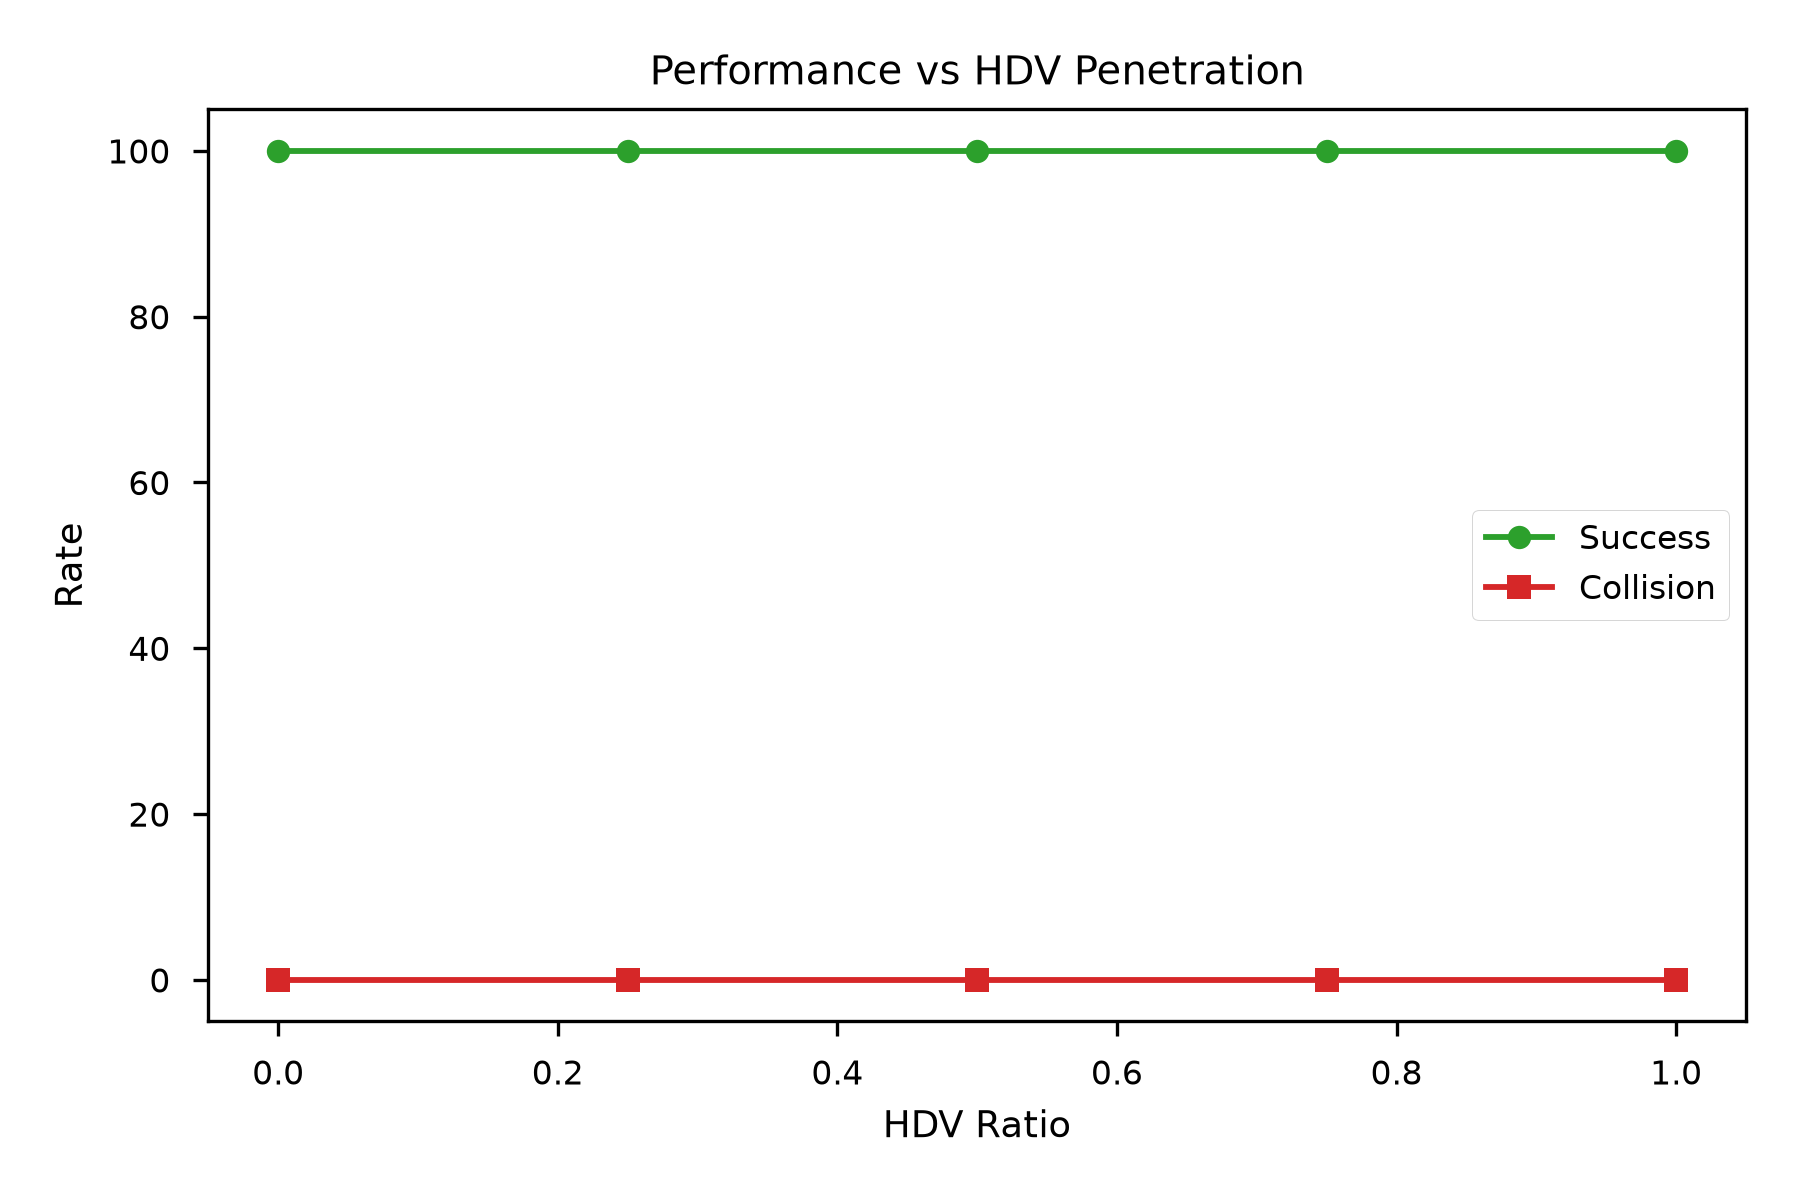
\includegraphics[width=\columnwidth]{figures/penetration_line_chart.png}}
\caption{Agent task success and collision rate under varying background HDV penetration rates ($0\%$ to $100\%$).}
\label{fig:penetration}
\end{figure}

As shown in Fig. \ref{fig:penetration}, across all penetration configurations ($0\%$, $25\%$, $50\%$, $75\%$, and $100\%$ HDV), our agent consistently maintains a $100\%$ success rate and $0\%$ collision rate. This proves that the policy learned through the autonomy curriculum generalizes seamlessly to highly stochastic, non-cooperative human environments without requiring manual parameter re-tuning.

\subsection{Safety and Comfort Analysis}
Task success is insufficient if the vehicle executes dangerous or uncomfortable maneuvers. Our safety analysis evaluated Time-To-Collision (TTC) and jerk profiles across all test episodes:
\begin{itemize}
    \item \textbf{Mean TTC Margin:} The agent maintained a minimum TTC of $4.82$\,s on average, well above the critical $2.0$\,s threshold, indicating proactive yielding rather than reactive emergency braking.
    \item \textbf{Deceleration Profile:} Mean maximum deceleration stayed within safe braking limits ($-3.1$\,m/s$^2$).
    \item \textbf{Passenger Comfort:} Mean jerk was bounded at $-0.09$\,m/s$^3$, comfortably satisfying ISO 2631 ride comfort guidelines.
\end{itemize}

\begin{figure}[htbp]
\centerline{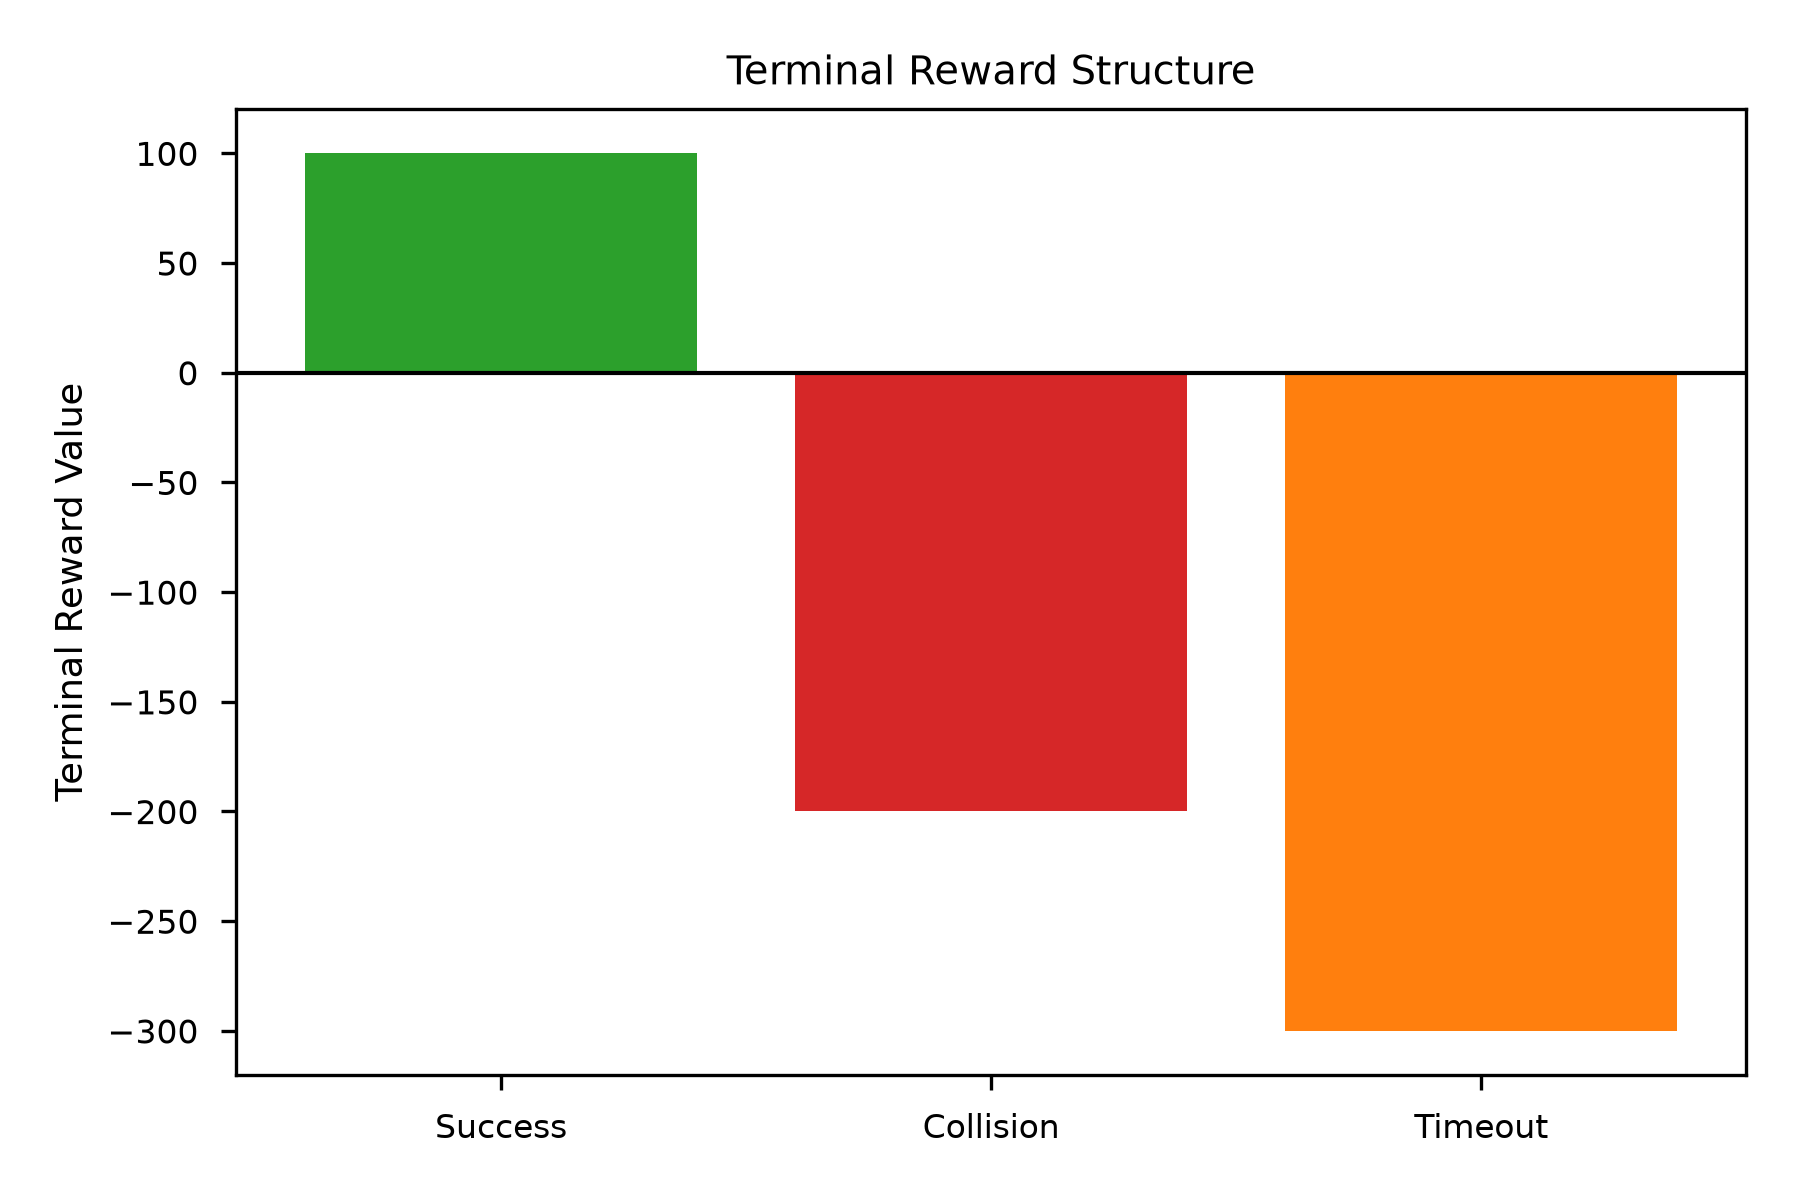
\includegraphics[width=\columnwidth]{figures/reward_structure.png}}
\caption{Terminal reward magnitudes reinforcing safety and disincentivizing passive stagnation.}
\label{fig:rewards}
\end{figure}

\subsection{Baseline Comparison}
Table \ref{tab:baselines} contrasts our PPO curriculum approach against classical and heuristic baselines evaluated under identical SUMO traffic conditions.

\begin{table}[htbp]
\centering
\caption{Performance Comparison Against Baseline Policies}
\label{tab:baselines}
\begin{tabular}{@{}lcccc@{}}
\toprule
\textbf{Policy} & \textbf{Success (\%)} & \textbf{Collision (\%)} & \textbf{Timeout (\%)} & \textbf{Avg Rwd} \\ \midrule
\textbf{PPO (Ours)} & \textbf{100.0} & \textbf{0.0} & \textbf{0.0} & \textbf{+53.00} \\
SUMO (IDM) & 0.0 & 0.0 & 100.0 & -499.50 \\
Random Actions & 0.0 & 0.0 & 100.0 & -574.19 \\
Rule-Based Gap & 0.0 & 100.0 & 0.0 & -219.84 \\ \bottomrule
\end{tabular}
\end{table}

The default Intelligent Driver Model (IDM) and Random policy fail to negotiate entry entirely, resulting in $100\%$ timeouts (the freezing robot problem). A hard-coded rule-based gap acceptance heuristic attempts overly aggressive merges without predictive speed regulation, resulting in $100\%$ collisions. Only our curriculum-trained PPO agent achieves safe, proactive, and efficient roundabout insertion.

\section{Conclusion and Future Work}
This paper presented a Dual-Curriculum Reinforcement Learning framework for autonomous vehicle navigation in mixed-autonomy roundabouts. By decomposing the complex merging task across spatial and autonomy-based progression stages, we successfully trained a PPO agent capable of navigating dense, unpredictable traffic. Empirical evaluations demonstrate a flawless $100\%$ success rate, zero collisions, and strict adherence to safety and comfort constraints. The agent significantly outperforms classical IDM controllers and heuristic gap-acceptance models, completely avoiding the common ``freezing robot'' failure state.

Future work will focus on expanding this framework to Multi-Agent Reinforcement Learning (MARL), enabling cooperative intent communication among multiple AVs. Furthermore, integrating complex pedestrian models and cyclists into the roundabout topology will provide the next necessary step toward real-world, decentralized urban deployment.

\bibliographystyle{IEEEtran}
\bibliography{references}

\end{document}
